\section{期望相关的不等式}

\paragraph{1. Jensen不等式} 先从一个简单的例子开始. 假设我们从$[1,99]$的范围内选取一个正方形的边长$X$, 问面积的期望是多少? 根据上面的公式, 我们知道$\Ep{X^2}= \int_{0}^{99} x^2 dx = 9950/3$. 

在式子变得复杂之后, 这样的运算就稍显麻烦. 能不能偷懒计算$\Ep{X}^2$代替上述的计算? 并不可以, 因为$\Ep{X}^2=50^2=2500.$ 但是我们可以看到大小关系: $\Ep{X^2}\geq \Ep{X}^2$. 并且可以证明它是对的: 
\begin{proof}
    考虑$Y=(X-\Ep{X})^2$, 随机变量$Y$非负, 意味着其期望也是非负的. 所以有
    $$
\begin{aligned}
0 \leq \mathbf{E}[Y] & =\mathbf{E}\left[(X-\mathbf{E}[X])^2\right] \\
& =\mathbf{E}\left[X^2-2 X \mathbf{E}[X]+(\mathbf{E}[X])^2\right] \\
& =\mathbf{E}\left[X^2\right]-2 \mathbf{E}[X \mathbf{E}[X]]+(\mathbf{E}[X])^2 \\
& =\mathbf{E}\left[X^2\right]-(\mathbf{E}[X])^2
\end{aligned}
$$
\end{proof}

\mn{-- 高数老师告诉过我, 高等数学里面和数学分析里面函数的凹凸性定义是相反的. 求偏导的时候求的顺序也是相反的. 那我应该相信谁?  \\ -- 相信定义. }
实际上, 这只是Jensen不等式的一个例子. Jensen不等式会告诉我们, 对于任意的一个凸函数$f$, 都会有$\Ep{f(X)}\geq f(\Ep{X})$. 

\begin{asidebox}
回顾凸函数: 一个函数$f:\mathbb R \to \mathbb R$是凸函数, 当且仅当$\forall x_1, x_2, 0\leq \lambda \leq 1$, 有$$
f\left(\lambda x_1+(1-\lambda) x_2\right) \leq \lambda f\left(x_1\right)+(1-\lambda) f\left(x_2\right) .
$$

并且我们知道, 如果 $f$ 是二次可微函数, 则 $f$ 是凸函数当且仅当 $f''(x)\geq 0$. 
\end{asidebox}

\begin{theorem}
    如果$f$是凸函数, 那么$\mathbf{E}[f(X)] \geq f(\mathbf{E}[X])$. 
\end{theorem}

\begin{proof}
    假设 $f$ 有Taylor 展开式. 令 $\mu=\mathbf{E}[X]$. 根据Taylor中值定理,存在一个值 $c$ 使得
$$
\begin{aligned}
f(x) & =f(\mu)+f^{\prime}(\mu)(x-\mu)+\frac{f^{\prime \prime}(c)(x-\mu)^2}{2} \\
& \geq f(\mu)+f^{\prime}(\mu)(x-\mu)
\end{aligned}
$$
由于$f$是凸函数, 得到 $f^{\prime \prime}(c)>0$ . 两边同时取期望, 得到: 
$$
\begin{aligned}
\mathbf{E}[f(X)] & \geq \mathbf{E}\left[f(\mu)+f^{\prime}(\mu)(X-\mu)\right] \\
& =\mathbf{E}[f(\mu)]+f^{\prime}(\mu)(\mathbf{E}[X]-\mu) \\
& =f(\mu)=f(\mathbf{E}[X]) .
\end{aligned}
$$
\end{proof}

\paragraph{2. Cauchy-Schwarz不等式}
这个不等式说的是下面的一个事情: 


\mn{这使我想到了线性代数的时候学习内积空间的时候的痛苦... }
对于随机变量  $ X, Y $, 我们有$ \mathbb{E}[|X Y|]^2 \leqslant \mathbb{E}\left[X^2\right] \mathbb{E}\left[Y^2\right]$
    
  
    
    首先考虑$\Ep{X^2} = \int_{-\infty}^{\infty} x^2 f_X(x), \Ep{X^2} = \int_{-\infty}^{\infty} y^2 f_Y(y)$. 为了方便起见, 不妨设$\Ep{X}, \Ep{Y}$都大于0. 假若我们引入新变量, 使得我们的$\tilde{X}, \tilde{Y}$的值都在 0到1之间: 
    $$
    \tilde{X}:= \frac{X}{\sqrt{\Ep{X^2}}},\tilde{Y}:= \frac{Y}{\sqrt{\Ep{Y^2}}} 
    $$
    这个时候由于任意的值有基本不等式, 故随机变量也要满足基本不等式描述的: $2|\tilde{X}\tilde{Y}|\leq \tilde{X^2}\tilde{Y^2}$. 对两边取期望, 有$2\Ep{\tilde{X}\tilde{Y}}\leq \Ep{\tilde{X^2}}\Ep{\tilde{Y^2}}=2$. 因此有$\Ep{\tilde{X}\tilde{Y}}\leq 1$, 自然
    $$
        \Ep{|X Y|}^2 = \mathbb{E}\left[X^2\right] \mathbb{E}\left[Y^2\right]
    $$ 

    \begin{asidebox}
        这个不等式我们在线性代数课程上面讲解向量的模的时候也有一个类似的不等式. 也就是如果一个线性空间$V$中$u,v\in V$, 那么有
        $$
        |\langle u, v\rangle| \leq\|u\|\|v\|.
        $$
        其中, $||\cdot||$是$\cdot$的范数. 

        向量的范数一般定义为$\sqrt{\langle v, v\rangle}$. 
    \end{asidebox}

\paragraph{3. Markov不等式} 概率和期望之间有什么联系? 在\cref{eg:expectation-calc}中, 我们了解到了期望计算和概率相联系的一种形式: $\Ep{X}=\int_0^\infty P(X>t) dt$. 自然的, $P(X>\epsilon)$和$\Ep{X}$有联系. 

\begin{theorem}
    Markov不等式: 
    $$
\forall \varepsilon>0, P(X>\varepsilon) \leqslant \frac{\mathbb{E}[X]}{\varepsilon}
$$
\end{theorem}

\begin{wrapfigure}{l}{0.6\textwidth}
    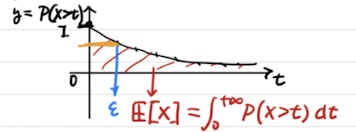
\includegraphics[width=0.6\textwidth]{fig/ch4/markov-ineq.jpg} 
    \caption{Markov不等式限制的方式}
    \label{fig:markov-ineq}
\end{wrapfigure}

\mn{-- 怎么说把这个东西切了就切了? 有点太粗暴了吧! \\ -- 实际上期望是它的一阶矩, 如果我们知道了更高阶的矩, 我们得到的信息就多了. }
我们采用最粗暴的限制限制手段. 如\cref{fig:markov-ineq}, 仅仅考虑$0\leq t\leq \epsilon, 0<y<P(x>\epsilon)$的部分. 因此, 我们可以得到证明: 
$$
\begin{aligned}
\mathbb{E}[x] & \geqslant \int_0^{\varepsilon} P(x>t) d t \\
& \geqslant \int_0^{\varepsilon} P(x>\varepsilon) d t \\
& =\varepsilon P(x>\varepsilon)
\end{aligned}
$$

于是我们可以得到想要的不等式. 